\chapter{Marco Teórico}

% Conceptos involucrados
% - Nuevas tecnologías consideradas
% - Metodologías de desarrollo
% - Algoritmos existentes
% - Arquitecturas estándar
% - Descripción de las soluciones existentes
% Concentra la mayor parte de las citas
% Alquien que conoce del tema podría saltearse este capítulo e igual comprender la memoria

\section{Ciencia de datos: espectroscopía astronómica}

Durante el siglo XIX nace la astrofísica moderna. Fue entonces que, por primera vez, se logró medir distancias estelares; que revelaron lo lejanos que se encuentran estos objetos de la tierra. Surgió, también en aquel siglo, la \textit{espectroscopía física}, que permitió la identificación de elementos químicos a través de \textit{líneas espectrales}. A partir de esto nace la química moderna, con el descubrimiento de la tabla periódica de los elementos. Gracias a estos avances es que, posteriormente, llega a surgir la mecánica cuántica en el siglo XX y, junto con ello, la clasificación espectral de las estrellas.

En el año 1814, el científico Joseph von Fraunhofer (1787 - 1826), mediante el uso de prismas de alta calidad construidos por él mismo, logró difractar un rayo de luz solar y proyectarlo hacia un muro blanco. Además de los colores característicos del arcoíris, observados de esta manera desde los tiempos de Newton, vio en la proyección resultante muchas líneas oscuras. Procedió, luego, a catalogar meticulosamente la longitud de onda exacta de cada una de estas líneas, que hasta el día de hoy se conocen como líneas de Fraunhofer, y asignó letras a las más notorias. De esta forma, Fraunhofer registró el primer espectro astronómico de alta resolución.

\begin{figure}[h!]
\begin{center}
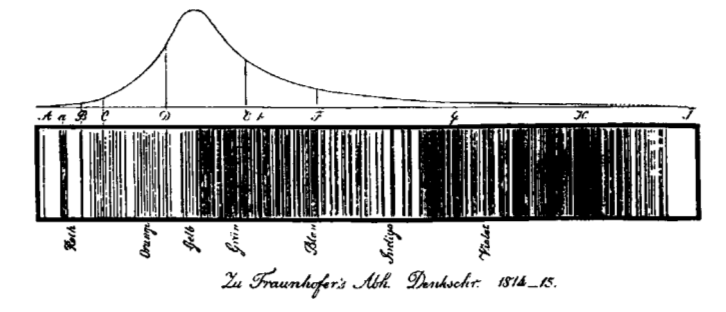
\includegraphics[width=14cm]{imagenes/fraunhofer_sun.png}
\end{center}
\vspace*{-5mm}
\caption{Espectro solar registrado por Fraunhofer.}
\label{fig:fraunhofer_sun}
\end{figure}

Posteriormente, procedió a realizar el mismo experimento, pero esta vez utilizando un rayo de luz proveniente de la estrella roja cercana Betelgeuse, y observó que el patrón de líneas oscuras cambiaba considerablemente. Fraunhofer concluyó correctamente que estas se encuentran de cierta forma relacionadas con la composición del objeto observado. En efecto, algunas de las líneas observadas por Fraunhofer se deben a las especies (e.g átomos, iones, moléculas) que componen la atmósfera terrestre.

Sin embargo, el gran paso en la comprensión general de las observaciones de Fraunhofer llegó a mediados del siglo XIX de la mano del trabajo de los científicos Gustav Kirchhoff (1824 - 1887) y Robert Bunsen (1811 - 1899), quienes estudiaron el color de la luz emitida al poner distintos metales en llamas. Al hacer esto, descubrieron que, en ciertos casos, la longitud de onda de la luz emitida coincidía exactamente con las líneas observadas por Fraunhofer. Estos experimentos demostraron que las líneas de Fraunhofer son una consecuencia directa de la composición atómica del sol.

En el siglo XX se llegó a comprender de manera más profunda la razón de la existencia de estas líneas, denominadas \textit{líneas espectrales}, gracias a la revolución que significó la llegada de la mecánica cuántica. Los desarrollos en materia de espectroscopía han estado, desde entonces, estrechamente ligados a los de aquel campo de la física.

Si se observa cuidadosamente ciertos objetos, tales como los planetas Marte o Júpiter, o estrellas tales como Betelgeuse, se puede apreciar que estos objetos tienden a tener un cierto color. Basta utilizar instrumentos de bajo poder resolutivo para separar la luz que llega desde estos objetos a la tierra en colores de amplio espectro. A su vez, el observar estos colores entrega información sobre la temperatura del objeto. Por ejemplo, las estrellas azules poseen mayor temperatura que las rojas. Objetos que emiten rayos X, como la corona solar, son muy calientes, mientras que objetos fríos emitirán radiación en longitudes de onda mayores; por ejemplo, en forma de ondas de radio.

La mejor forma de obtener información astrofísica detallada de objetos del cielo es mediante observaciones de alta resolución espectral. Observaciones llevados a cabo con estos equipos con tal capacidad permiten obtener, no solamente la posición central de una línea dentro del espectro, sino también su forma. Mediante este procedimiento se puede inferir propiedades del objeto, tales como su composición química, su temperatura, la abundancia de las especies que lo componen y que se encuentran emitiendo radiación, el movimiento de las especies y del objeto en sí, la presión y densidad local, el campo magnético presente, entre otros.

Esto se lleva a cabo con equipos de alto poder resolutivo y sensibilidad. Dos ejemplos de estos son, el telescopio óptico SDSS que se encuentra en el Apache Point Observatory (APO, ubicado en Nuevo México, Estados Unidos) y con el cual se lleva a cabo el \textit{Sloan Digital Sky Survey (SDSS)}; y, en mayor medida, el interferómetro radioastronómico \textit{Atacama Large Millimeter/submillimeter Array (ALMA)} ubicado en el norte de Chile.

\subsection{Atacama Large Millimeter Array (ALMA)}

El \textit{Atacama Large Millimeter Array (ALMA)} es un interferómetro de señales de radio ubicado en el desierto de Atacama, en el norte de Chile. Es un proyecto llevado a cabo mediante una asociación de organizaciones de Norteamérica, Europa y el Este de Asia. Comenzó sus observaciones científicas en la segunda mitad del año 2011. Es, por lejor, el mayor y más importante radiotelescopio construido hasta la fecha. Se encuentra realizando observaciones preliminares desde marzo del año 2013, y se espera que que opere al cien por ciento de su capacidad desde marzo del 2017.

ALMA realiza observaciones captando radiación electromagnética proveniente del espacio en bandas milimétricas y submilimétricas en sus longitudes de onda, que corresponden a ondas de radio. Debido a que en condiciones normales la humedad del ambiente y del cielo absorbe gran parte de este tipo de radiación, es crucial para el funcionamiento de los telescopios el estar ubicados en un lugar seco; y el más idóneo en ese sentido es, sin dudas, el llano de Chajnantor en el desierto de Atacama, a más de 5000 metros de altura.

Debido al diseño de ALMA, en muchas de sus observaciones se detectará una abundancia de líneas espectrales; lo cual puede ser un resultado complementario al objetivo principal de una observación en particular, y por ende, puede no ser analizado por el o la astrónomo(a) que lo propuso.

Con el tiempo se espera ocurra una eventual acumulación de grandes cantidades de datos espectrales de ALMA. Esto abre la oportunidad de desarrollar nuevas técnicas de estudio basados en la minería de datos u otras técnicas de computación poco usadas por los astrónomos. De ahí que en el presente trabajo se busque implementar algoritmos de aprendizaje de reglas de asociación, o \textit{Association Rule Learning (ARL)}, para el estudio masivo de datos espectroscópicos

Gran parte de los datos obtenidos desde ALMA son guardados en estructuras de datos llamadas cubos de datos tipo ALMA (o \textit{ALMA Data Cubes})\label{fig:data_cube}, que contienen información de distintos puntos de observación del cielo a distintas frecuencias. Los cubos de datos tipo ALMA, como estructura de datos, contienen valores indexados en tres coordenadas. Dos de las coordenadas son espaciales, y corresponden al equivalente a una imagen normal de dos dimensiones, en el sentido que describen puntos del cielo (o del espacio observable desde la tierra). La tercera coordenada corresponde al rango de frecuencias en el que se está detectando radiación electromagnética. Por lo tanto, si se fijan las dos coordenadas espaciales (se fija un punto en el espacio) y se extraen todos los valores en la tercera coordenada de aquel punto, se obtiene el espectro de frecuencias observado en ese punto del espacio.

\begin{figure}[h!]
\begin{center}
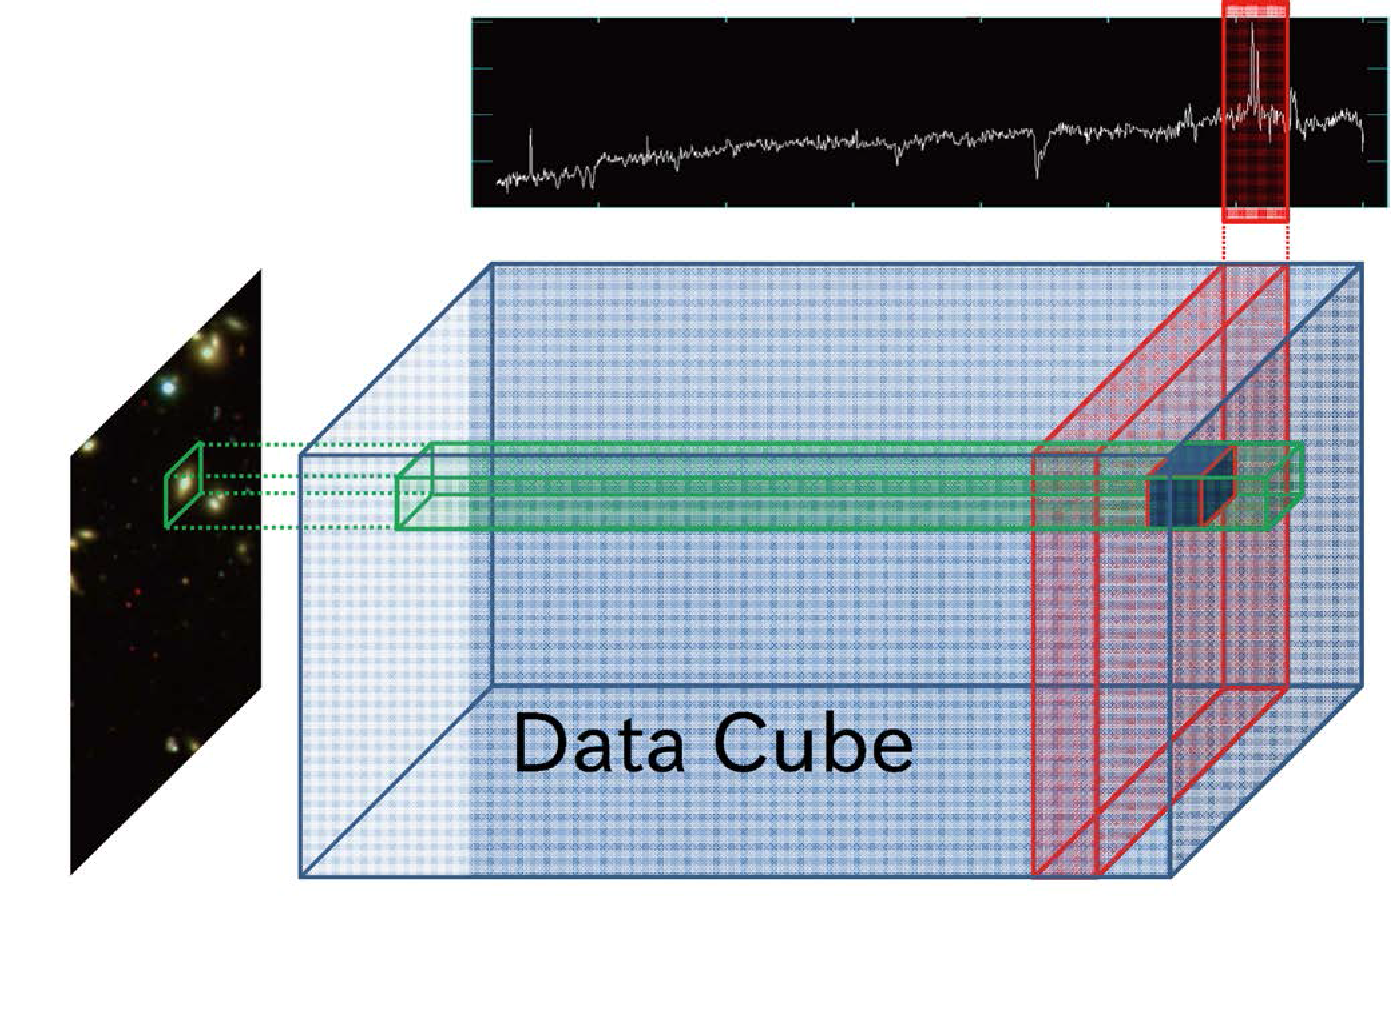
\includegraphics[width=14cm]{imagenes/data_cube.png}
\end{center}
\vspace*{-5mm}
\caption{Representación gráfica de un cubo de datos tipo ALMA. Dos de sus cordenadas son espaciales mientras la tercera corresponde al dominio de las frecuencias.}
\label{fig:data_cube}
\end{figure}

A partir de ALMA se generan enormes cantidades de datos (actualmente cerca el orden de 1 TeraByte al día), los cuales necesariamente deben procesarse por parte de sistemas automatizados de extracción y análisis con el fin de facilitar a los investigadores el inferir información útil a partir de estos.

\subsection{Sloan Digital Sky Survey (SDSS)}

Dado que se espera obtener datos de ALMA para el uso de técnicas tales como el aprendizaje de reglas de asociación a partir del año 2017, se requiere una base de datos espectroscópicos pre-existente con el fin de poner a prueba el sistema desarrollado en el presente trabajo.

El \textit{Sloan Digital Sky Survey (SDSS)} es un proyecto de inspección y estudio del espacio llevado a cabo mediante el uso de un telescopio óptico ubicado en el observatorio Apache Point (APO), Nuevo México, Estados Unidos. La recolección de datos comenzó en el año 2000, y las imágenes finales de los datos publicados cubren un 35\% del cielo, con observaciones fotométricas de 500 millones de objetos y espectros ópticos de 1 millón de objetos.

Los espectros del SDSS cubren desde 3600 a 10400 Angstroms ({\AA})\footnote{\url{https://www.sdss3.org/instruments/boss_spectrograph.php\#Parameters}} con una resolución de 1 {\AA}\footnote{$1\,\text{{\AA}} = 10^{-10}\,m = 10^{-1}\,nm$}. Los objetos estudiados son principalmente galaxias, incluyendo \textit{quásares} y \textit{AGN} (un 80\% del total de datos), y el resto son estrellas de distinto tipo (20\% del total) cuyos espectros se encuentran dominados por muchas líneas de absorción. Los espectros de regiones de gas o de galaxias, por otra parte, poseen pocas líneas de absorción. El SDSS tiene en sus catálogos un universo de casi 50 líneas espectrales posibles, presentes dentro de su rango de detección.

Los datos de SDSS se hacen disponibles mediante publicaciones regulares o \textit{data releases} a través de internet. La última publicación llevada a cabo fue la correspondiente al data release 10 (DR10), con fecha de julio del 2013. Los datos de todos los data releases se encuentran en un servidor \textit{Microsoft SQL Server} y pueden accederse mediante diversas interfaces o APIs presentes en el sitio web de SDSS. En particular, existe una interfaz web llamada \textit{CasJobs} que permite realizar consultas en lenguaje \textit{SQL} a un servidor que encola la petición, la ejecuta y guarda los resultados en una base de datos asignada al usuario.

Para probar los algoritmos y el sistema implementados en el presente trabajo, en particular, se utilizó el \textit{data release 7 (DR7)} como fuente de datos.

\section{Reglas de asociación}

El aprendizaje mediante reglas de asociación, o \textit{Association Rule learning (ARL)}, es sin lugar a dudas uno de los métodos más populares y mejor estudiados dentro de la minería de datos. Basta para ello ver que el artículo seminal de Agrawal et al.\cite{agrawal1993mining}, donde se sentaron las bases de la teoría subyacente, es uno de los más citados del área; según el catálogo y herramienta de búsqueda de publicaciones científicas \textit{Google Scholar}.

La motivación principal de ARL en su concepción fue el encontrar relaciones lógicas entre los artículos adquiridos por usuarios en puntos de venta del tipo \textit{"Si un cliente compra los artículos A y B, entonces es muy probable que también compre el artículo C"}. Sin embargo, la teoría de fondo que se desarrolló con el tiempo tiene una gran cantidad de aplicaciones en los más diversos ámbitos.

\subsection{Definición formal}

Sea $\mathcal{I} = \{i_1,\,i_2,\,i_3,\,\ldots ,\,i_n\}$ un universo de ítemes posibles. Se denomina, entonces a un conjunto $X \subseteq \mathcal{I}$ como \textit{conjunto de ítemes} o \textit{itemset}. Se tiene, además un conjunto de transacciones $\mathcal{T} = \{T_1,\,T_2,\,\ldots,\,T_m\}$, donde $T_i \subseteq \mathcal{I}, \; \forall i \in {[1,m]}$. Dados un conjunto de ítemes $X$ y una transacción $T_i$, se dice que la trasacción $T_i$ \textit{satisface} $X$ si y solo si $X \subseteq I_i$.

Una \textit{regla de asociación} es, entonces, una relación (más específicamente, una implicancia) entre dos conjuntos de la forma $X \Rightarrow Y$, donde $X \subset \mathcal{I}$, $Y \subset \mathcal{I}$, y $X \cap Y = \emptyset$. A $X$ se denomina el \textit{antecedente} de la regla y a $Y$ se denomina el \textit{consecuente} de la regla.

Existen una serie de medidas para cuantificar la relevancia de una regla de asociación. A continuación se define algunas de ellas.

El \textit{soporte} de un conjunto de ítemes $X$, o $\mathit{supp}(X)$, se define como $$\mathit{supp}(X) = \frac{|\mathcal{T}_X|}{|\mathcal{T}|} \quad \text{, tal que} \quad \mathcal{T}_X = \{T \in \mathcal{T} \, : \, X \subset T \}\text{,}$$ donde $|X|$, cuando $X$ es un conjunto finito cualquiera, significa el número de elementos que posee el conjunto. Vale decir, el soporte corresponde a la fracción del total de transacciones en la que está presente el conjunto.

A su vez, el soporte de una regla de asociación $X \Rightarrow Y$, o $\mathit{supp}(X \Rightarrow Y)$, se define como $$\mathit{supp}(X \Rightarrow Y) = \mathit{supp}(X \cup Y)\text{,}$$ vale decir, corresponde a la fracción del total de transacciones en las cuales está presente tanto el antecedente como el consecuente de la regla simultáneamente\footnote{Debe tenerse en mente que la expresión $mathit{supp}(X \cup Y)$ indica la fracción del total de transacciones en las cuales está presente \textbf{tanto} el antecedente como el consecuente de la regla \textbf{simultáneamente}, y \textbf{no} de aquellas en las cuales está presente el antecedente \textbf{o} el consecuente. El argumento del soporte $\mathit{supp}$ es un conjunto de ``pre-condiciones", y, por lo tanto, se vuelve más restrictivo en la medida que su cardinalidad aumenta.}.

La \textit{confianza} de una regla de asociación $X \Rightarrow Y$, denotada por $\mathit{conf}(X \Rightarrow Y)$, se define como $$\mathit{conf}(X \Rightarrow Y) = \frac{\mathit{supp}(X \cup Y)}{\mathit{supp}(X)}\text{,}$$ es decir, indica en qué fracción de las transacciones en las cuales está presente el antecedente la regla se cumple (i.e. está presente también el consecuente de la regla). Debido al uso frecuente de esta medida de relevancia, resulta usual el expresar una regla de asociación mediante la notación $$X \Rightarrow Y \, \Big| \, c$$ donde $c = \mathit{conf}(X \Rightarrow Y)$.

El \textit{lift} de una regla de asociación $X \Rightarrow Y$, denotado por $\mathit{lift}(X \Rightarrow Y)$, se define como $$\mathit{lift}(X \Rightarrow Y) = \frac{\mathit{conf}(X \Rightarrow Y)}{\mathit{supp}(Y)} = \frac{\mathit{supp}(X \cup Y)}{\mathit{supp}(X) \times \mathit{supp}(Y)}\text{.}$$ La intuición detrás del concepto de lift tiene lugar al interpretar las medidas descritas anteriormente desde un punto de vista probabilístico. Tomando el conjunto $\mathcal{T}$ como un universo de posibles resultados, o espacio muestral, se tiene que $$\mathit{supp}(X) = P(X) \quad \text{y} \quad \mathit{conf}(X \Rightarrow Y) = P(Y| X)\text{.}$$ Desde este punto de vista, la medida de lift indica qué tan bien la presencia del antecedente de una regla lograría predecir la presencia del consecuente. Por lo tanto, si la presencia del antecedente y del consecuente en una transacción cualquiera son eventos estadísticamente independientes (i.e. la ocurrencia de uno no afecta la probabilidad de que el otro ocurra), se tendrá que $\mathit{lift}(X \Rightarrow Y) = 1$; y este valor irá variando en la medida que ambos eventos sean más dependientes entre sí.

Por ejemplo, supongamos que se tiene el siguiente conjunto de transacciones

\begin{tabular}{l l}
\textbf{TID} & \textbf{Items} \\
1 & $a$, $c$ \\
2 & $a$, $d$ \\
3 & $b$, $c$ \\
4 & $b$, $d$ \\
\end{tabular}

donde \textit{TID} es el número identificador de la transacción. Luego, para este caso, se tiene que $$\mathit{lift}(\{a\} \Rightarrow \{c\}) = \frac{\mathit{supp}(\{a\} \cup \{c\})}{\mathit{supp}(\{a\}) \times \mathit{supp}(\{c\})} = \frac{1/4}{1/2 \times 1/2} = 1\text{,}$$ lo cual indica que la que la ocurrencia de que una transacción cualquiera satisfaga $\{a\}$ es estadísticamente independiente de que una transacción cualquiera satisfaga $\{b\}$.

En cambio, en el siguiente conjunto de transacciones

\begin{tabular}{l l}
\textbf{TID} & \textbf{Items} \\
1 & $a$, $c$ \\
2 & $a$, $d$ \\
3 & $b$, $c$ \\
4 & $b$, $c$ \\
\end{tabular}

se tiene que $$\mathit{lift}(\{a\} \Rightarrow \{c\}) = \frac{\mathit{supp}(\{a\} \cup \{c\})}{\mathit{supp}(\{a\}) \times \mathit{supp}(\{c\})} = \frac{1/4}{1/2 \times 3/4} = 2/3 < 1\text{,}$$ lo cual quiere decir que hay una mayor razón de transacciones que satisfacen $\{c\}$ dentro del total de transacciones que dentro del conjunto de transacciones que satisfacen $\{a\}$.

Finalmente, en el conjunto de transacciones

\begin{tabular}{l l}
\textbf{TID} & \textbf{Items} \\
1 & $a$, $c$ \\
2 & $a$, $d$ \\
3 & $b$, $d$ \\
4 & $b$, $d$ \\
\end{tabular}

se cumple que $$\mathit{lift}(\{a\} \Rightarrow \{c\}) = \frac{\mathit{supp}(\{a\} \cup \{c\})}{\mathit{supp}(\{a\}) \times \mathit{supp}(\{c\})} = \frac{1/4}{1/2 \times 1/4} = 2 > 1\text{,}$$ lo cual indica que hay una mayor razón de transacciones que satisfacen $\{c\}$ dentro del conjunto de transacciones que satisfacen $\{a\}$ que dentro del total de transacciones.

\subsection{Algoritmos principales}

\subsubsection{Algoritmo \textit{Apriori}}

En el mismo artículo seminal de ARL por Agrawal et al.\cite{agrawal1993mining}, se presentó el algoritmo \textit{Apriori}. Este algoritmo hace uso de las propiedades de clausura descendiente de la frecuencia de los conjuntos con respecto a sus subconjuntos con el fin de optimizar el proceso de generación de conjuntos de ítemes frecuentes.

El algoritmo \textit{Apriori} recibe como entrada un conjunto de transacciones, y tiene como objetivo encontrar y retornar todos aquellos conjuntos presentes que cumplan con el requisito de soporte mínimo indicado, también llamados \textit{conjuntos frecuentes}.

Por ejemplo, supongamos que se cuenta con el un conjunto de transacciones, y que cada una contiene ítemes pertenecientes a un universo de solo 4 elementos posibles, $\mathcal{I} = \{0,\,1,\,2,\,3\}$. Luego, en principio, para extraer los conjuntos frecuentes a partir de estas transacciones, por cada uno de los conjuntos que es posible generar con este universo de 4 ítemes posibles (llamados \textit{conjuntos candidatos}), se debe recorrer cada una de las transacciones, ver si la transaccion satisface este conjunto, y de ser así incrementar un contador. Luego de terminar este proceso para cada uno de los conjuntos posibles, se tendrá el número de veces que cada uno de estos se encuentra dentro del conjunto de transacciones, y teniendo el número total de estas, se puede obtener de forma directa el soporte de estos conjuntos.

\missingfigure{Grafo con los conjuntos generados a partir de un universo de 4 ítemes posibles}

El problema radica en que el número de conjuntos candidatos crece de manera exponencial en el número de ítemes del universo posible. En efecto, si el número de ítemes del universo es $n$, entonces a partir de este es posible generar $2^n+1$ conjuntos. Por tanto, para un universo de 100 elementos, existen nada menos que $1.26\times10^{30}$ conjuntos candidatos; y debe, por tanto, recorrerse el total de transacciones este número de veces.

No obstante, es posible reducir el número de conjuntos candidatos utilizando la propiedad de \textit{clausura descendiente} de los conjuntos frecuentes, tambien llamado \textit{principio Apriori}. Esta propiedad asegura que si un conjunto dado es, en efecto, frecuente, entonces necesariamente todos sus subconjuntos también lo son. O, expresado de forma recíproca, si un conjunto dado resulta no ser frecuente, entonces necesariamente todos sus superconjuntos tampoco lo son. Esta última expresión es la que resulta más relevante para nuestro caso. Esto implica que luego de generar un conjunto candidato y verificar si es frecuente verificando el número de transacciones que lo satisfacen, si se comprueba que este conjunto no es frecuente (vale decir, no cumple con el requisito de soporte mínimo), entonces necesariamente ninguno de sus conjuntos posibles que lo contienen será frecuente, y por tanto no será necesario obtener sus soportes correspondientes contando el número de transacciones que los satisfacen.

\missingfigure{Grafo igual al anterior, pero que muestra cuales de los conjuntos necesariamente no son frecuentes si uno de ellos resulta no serlo.}

Esta propiedad permite reducir considerablemente el número de conjuntos candidatos y, por tanto, optimizar el algoritmo final; ya que no será necesario recorrer el total de transacciones tantas veces como se planteó originalmente. Para poder utilizar esta propiedad y beneficiarse de la optimización correspondiente, es necesario generar los conjuntos candidatos comenzando por aquellos que poseen menos elementos, y a partir de estos generar todos los superconjuntos posibles.

El algoritmo \textit{Apriori}, por lo tanto, en terminos generales resulta ser el siguiente

\begin{algorithm}[H]
\DontPrintSemicolon
\KwData{Conjunto de transacciones $\mathcal{T}$}
\KwResult{Conjunto de ítemes frecuentes $\mathcal{L}$}
$\mathcal{L}_1 \leftarrow \{\text{conjuntos de 1 solo ítem}\}$\;
\For{$k = 2; \, L_{k-1} \neq \emptyset; \, {k++}$}{
	$C_k = \texttt{apriori-gen}(L_{k-1})$\;
	\For{transacciones $T \in \mathcal{T}$}{
	$\mathcal{C}_T = \texttt{subset}(\mathcal{C}_k,\,T)$\;
	\For{candidatos $C \in \mathcal{C}_t$}{
	$\text{C.count} \leftarrow \text{C.count} + 1$\;
	}
	}
	$\mathcal{L}_k = \{C \in \mathcal{C}_k \, : \, \text{C.count} \geq \text{minsup}\}$\;
}
$\mathcal{L} \leftarrow \bigcup_k \, \mathcal{L}_k$\;
\caption{Algoritmo \textit{Apriori}}
\end{algorithm}

Donde $\mathcal{L}_k$ corresponde a la colección de conjuntos frecuentes con $k$ elementos, los cuales tienen un contador asociado; y $\mathcal{C}_k$ consiste en la colección de conjuntos candidatos con $k$ elementos, que tienen también un contador asociado. La función \texttt{apriori-gen} es la encargada de generar la colección de conjuntos frecuentes de tamaño $k$ a partir de la colección de conjuntos candidatos datos de tamaño $k$. La función \texttt{subset} se encarga de recibir una colección de conjuntos de ítemes frecuentes $\mathcal{C}_k$ y una transacción $T$ y de retornar una colección de ítemes $\mathcal{C}_T = \{C \in \mathcal{C}_k \, : \, C \subseteq T\}$.

La teoría indica que la complejidad del algoritmo Apriori se encuentra está acotada por $\mathcal{O}(\mathcal{C}_{\mathit{sum}} \times |\mathcal{T}|)$, donde $\mathcal{C}_{\mathit{sum}}$ es la suma de los tamaños del total de conjuntos candidatos considerados y $|\mathcal{T}|)$ denota el tamaño del conjunto de transacciones.

\subsubsection{Algoritmo \textit{FP-Growth}}

Más recientemente, Han et al. introdujeron el uso de una estructura de datos llamada \textit{Frequent Pattern Tree}\cite{han2004mining} en la extracción de conjuntos de ítemes frecuentes a partir de conjuntos de transacciones. Con esto dieron origen al algoritmo \textit{FP-Growth}.

Un \textit{Frequent Pattern Tree (FP-Tree)} es una estructura de datos de tipo árbol, que consiste en un nodo raíz que tiene como sus hijos a \textit{sub-árboles de prefijos de ítems}. Cada nodo del \textit{sub-árbol de prefijo de ítem} contiene tres campos: el nombre del ítem al cual el nodo representa, un contador que registra el número de transacciones que satisfacen la rama del árbol que va de la raíz hasta este nodo, y un puntero al siguiente nodo del FP-Tree que contenga el mismo nombre de ítem o un puntero vacío si no existe tal nodo.

A su vez, el FP-Tree posee una estructura de datos auxiliar denominada \textit{tabla de encabezados}. Cada entrada en esta tabla posee dos campos. El primero es el nombre del ítem y el segundo es un puntero al primer nodo del FP-Tree que posee el mismo nombre de ítem.

Supongamos, por ejemplo, que se cuenta con el siguiente conjunto de transacciones:

\begin{tabular}{l l}
\textbf{TID} & \textbf{Ítemes} \\
1 & $r$, $z$, $h$, $j$, $p$ \\
2 & $z$, $y$, $x$, $w$, $v$, $u$, $t$, $s$ \\
3 & $z$ \\
4 & $r$, $x$, $n$, $o$, $s$ \\
5 & $y$, $r$, $x$, $z$, $q$, $t$, $p$ \\
6 & $y$, $z$, $x$, $e$, $q$, $s$, $t$, $m$ \\
\end{tabular}

Supongamos, entonces que se desea extraer de estas transacciones aquellos conjuntos frecuentes que cumplan un soporte mínimo de 0.5. El procedimiento para generar el FP-Tree es, entonces, el siguiente. En primer lugar, se extrae a partir de las transacciones todos los ítemes presentes y se ordenan por orden de frecuencia. En este caso, el resultado es el conjunto $I = \{z, \, r, \, x, \, y, \, s, \, t, \, p, \, q, \, h, \, j, \, w, \, v, \, u, \, n, \, o, \, e, \, m\}$. Luego, se elimina de este conjunto todos aquellos ítemes que no cumplan con el requisito mínimo de soporte deseado, obteniendo como resultado $I = \{z, \, r, \, x, \, y, \, s, \, t\}$

Luego, se hace lo mismo con los ítemes de las transacciones, obteniendo el siguiente resultado

\begin{tabular}{l l l}
\textbf{TID} & \textbf{Ítemes} & \textbf{Ítemes ordenados y filtrados} \\
1 & $r$, $z$, $h$, $j$, $p$ & $z$, $r$ \\
2 & $z$, $y$, $x$, $w$, $v$, $u$, $t$, $s$ & $z$, $x$, $y$, $s$, $t$ \\
3 & $z$ & $z$ \\
4 & $r$, $x$, $n$, $o$, $s$ & $x$, $s$, $r$ \\
5 & $y$, $r$, $x$, $z$, $q$, $t$, $p$ & $z$, $x$, $y$, $r$, $t$ \\
6 & $y$, $z$, $x$, $e$, $q$, $s$, $t$, $m$ & $z$, $x$, $y$, $s$, $t$ \\
\end{tabular}

Una vez listo esto, puede comenzarse con el procedimiento de construcción del árbol en sí. Se comienza por insertar el nodo raíz, cuyo nombre es vacío o \textit{null}. Luego se comienza a añadir los conjuntos frecuentes a partir de las transacciones con ítemes ordenados y filtrados. Estas son sucesivamente añadidas al árbol de tal manera que cada ítem resulte ser hijo del ítem anterior según el orden en que se encuentra en la transacción. Ahora bien, si el ítem a añadir ya se encuentra presente en una cierta posición dentro de el árbol, entonces en vez de agregar un nuevo nodo con el mismo nombre, simplemente se incrementa el contador del nodo ya existente y se inserta el siguiente ítem en la transacción como hijo de este.

\missingfigure{Proceso de construcción del FP-Tree del ejemplo}

En términos generales, el algoritmo final de generación de FP-Tree es como sigue

\missingfigure{FP-Tree y headertables resultantes del ejemplo}

Luego, se procede a extraer los conjuntos frecuentes a partir del FP-Tree de la siguiente manera

\subsection{Otros algoritmos, implementaciones y aplicaciones}

Posteriormente, Agrawal et al. presentaron el algoritmo \textit{AprioriTid}, cuyas mejores características fueron combinadas con el algoritmo \textit{Apriori} para crear el algoritmo \textit{AprioriHybrid}, de orden de complejidad lineal en el número de transacciones\cite{agrawal1994fast}. Luego se han realizado más desarrollos en ARL orientado a transacciones secuenciales de clientes de puntos de ventas\cite{agrawal1995mining}.

Savasere et al. introdujeron el algoritmo \textit{Partition}\cite{savasere1995efficient} con el fin de extraer reglas de asociación en base de datos, el cual presenta reducciones en las operaciones de la CPU y de entrada/salida, y que además facilita la paralelización. Posteriormente se creó el algoritmo \textit{Dynamic Itemset Counting (DIC)}\cite{brin1997dynamic}, que realiza menos lecturas sobre los datos que los algoritmos previos, y que utiliza la métrica de \textit{Convicción} a la hora de generar reglas de asociación. Luego, Park et al. presentaron un algoritmo que hace uso de funciones de Hashing con el fin de generar reglas candidatas\cite{park1995effective}. Se han realizado, también, adaptaciones de los algoritmos previos con el fin de realizar ARL en datos de tipo cuantitativo\cite{srikant1996mining}.

Esfuerzos posteriores se han realizado con el fin de profundizar en los fundamentos teóricos subyacentes en ARL (e.g. definiendo el conjunto de posibles ítemes como una estructura algebráica llamada \textit{retículo})\cite{zaki1998theoretical}, y con el fin de extender la noción de reglas de asociación a correlaciones\cite{brin1997beyond}.

Luego de esto, se han hecho numerosas implementaciones y optimizaciones a los algoritmos más utilizados en ARL, como, por ejemplo, el algoritmo Apriori\cite{bodon2010fast}; así como implementaciones que facilitan el mantener la privacidad de cada una de las fuentes de datos que participan en el proceso\cite{evfimievski2004privacy}.

Desde su concepción, el método de ARL ha sido aplicado en numerosas áreas, tales como la detección de intrusiones\cite{lee2000framework} y anomalías\cite{patcha2007overview}\cite{chandola2009anomaly}, educación\cite{romero2007educational}\cite{romero2008data}, química\cite{dehaspe1998finding}, privacidad de datos\cite{ghinita2008private}, búsqueda en la web\cite{ferragina2008personalized}, tráfico en redes\cite{estan2003automatically}, computación social\cite{li2008tag}, búsqueda semántica\cite{cohen2007associative}, biología\cite{kramer2001molecular}\cite{carmona2007genecodis}, salud\cite{karabatak2009expert}\cite{chaves2011efficient}, medios de comunicación\cite{davidson2010youtube}\cite{kobilarov2009media}, y la investigación forense\cite{iqbal2013unified}. Junto con esto, se han realizado numerosas investigaciones sobre el estado actual de ARL y sus posibles desarrollos a futuro dentro del marco de métodos automatizados de generación de conocimiento\cite{han2007frequent}.

Si bien existen numerosos esfuerzos por utilizar minería de datos y Machine Learning en diversos ámbitos de la astronomía (en particular, en detección, clasificación y caracterización de líneas moleculares en espectros de emisión\cite{vskoda2011searching}), hasta la fecha no se ha propuesto abiertamente el uso de ARL sobre datos extraídos de espectros de frecuencia.

Sin embargo, se han realizado avances en ampliar los conceptos subyacentes en ARL con el fin de aplicar el método en campos más diversos\cite{brin1997beyond}. Específicamente, una rama de investigación ha desarrollado lo que se denomina \textit{Weighted Association Rule Learning}\cite{wang2000efficient}\cite{cai1998mining}. Este método permite asociar medidas de interés arbitrario a priori a ciertos conjuntos de datos. Si bien esto hace que se pierdan propiedades de clausura que son útiles a la hora de generar algoritmos eficientes, también permite trabajar con distintos conjuntos de transacciones sin que las reglas generadas estos dependan exclusivamente de su soporte u otras medidas estándar.

